\chapter{Applying Rapid Whole-Genome Sequencing To Predict Phenotypic Antimicrobial Susceptibility Testing Results among Carbapenem-Resistant \textit{Klebsiella pneumoniae} Clinical Isolates}
\label{chap:amr}

\textbf{Portions of this chapter originally appeared in:} \\
Tamma PD, Fan Y, Bergman Y, Pertea G, Kazmi AQ, Lewis S, et al. Applying Rapid Whole-Genome Sequencing To Predict Phenotypic Antimicrobial Susceptibility Testing Results among Carbapenem-Resistant \textit{Klebsiella pneumoniae} Clinical Isolates 2019;63. https://doi.org/10.1128/AAC.01923-18

\section{Abstract}
\label{sec:abstract}

Standard antimicrobial susceptibility testing (AST) approaches lead to delays in the selection of optimal antimicrobial therapy. Here, we sought to determine the accuracy of antimicrobial resistance (AMR) determinants identified by Nanopore whole-genome sequencing in predicting AST results. Using a cohort of 40 clinical isolates (21 carbapenemase-producing carbapenem-resistant Klebsiella pneumoniae, 10 non-carbapenemase-producing carbapenem-resistant K. pneumoniae, and 9 carbapenem-susceptible K. pneumoniae isolates), three separate sequencing and analysis pipelines were performed, as follows: (i) a real-time Nanopore analysis approach identifying acquired AMR genes, (ii) an assembly-based Nanopore approach identifying acquired AMR genes and chromosomal mutations, and (iii) an approach using short-read correction of Nanopore assemblies. The short-read correction of Nanopore assemblies served as the reference standard to determine the accuracy of Nanopore sequencing results. With the real-time analysis approach, full annotation of acquired AMR genes occurred within 8 h from subcultured isolates. Assemblies sufficient for full resistance gene and single-nucleotide polymorphism annotation were available within 14 h from subcultured isolates. The overall agreement of genotypic results and anticipated AST results for the 40 K. pneumoniae isolates was 77\% (range, 30\% to 100\%) and 92\% (range, 80\% to 100\%) for the real-time approach and the assembly approach, respectively. Evaluating the patients contributing the 40 isolates, the real-time approach and assembly approach could shorten the median time to effective antibiotic therapy by 20 h and 26 h, respectively, compared to standard AST. Nanopore sequencing offers a rapid approach to both accurately identify resistance mechanisms and to predict AST results for K. pneumoniae isolates. Bioinformatics improvements enabling real-time alignment, coupled with rapid extraction and library preparation, will further enhance the accuracy and workflow of the Nanopore real-time approach.

\section{Introduction}
\label{sec:intro}

Whole-genome sequencing (WGS) has enabled notable advancements to the field of infectious diseases, such as an improved understanding of transmission dynamics and outbreak analysis (1). An exciting possibility from this technology is the ability to predict antimicrobial susceptibility testing (AST) results based on the identification of acquired resistance genes and/or chromosomal mutations (2).

Currently, there are several shortcomings with standard approaches to AST, particularly as they relate to multidrug-resistant Gram-negative (MDRGN) organisms. First, AST results are reported approximately 48 to 72 h after the time of culture collection, potentially leading to delays in appropriate empirical antibiotic therapy (3). Second, automated AST panels are limited in the number of antibiotic agents included. For agents that frequently need to be considered for highly drug-resistant pathogens (e.g., colistin, tigecycline, ceftazidime-avibactam, etc.) and newer agents in later phases of development that are unlikely to be routinely included in AST panels for the foreseeable future, there are additional delays in AST determination. As it is generally not evident at the time antibiotics are initiated that a patient will be infected with an MDRGN organism, susceptibility testing for these last-resort agents occurs subsequent to, and not simultaneously with, automated AST testing. Third, standard AST reporting does not include identification of resistance mechanisms (e.g., carbapenemases, extended-spectrum β-lactamases [ESBLs], etc.), which can be important for guiding antibiotic treatment decisions, as in vitro activity does not always translate to in vivo activity (4). WGS can potentially alleviate many of these concerns by offering the potential to predict AST results by identifying the presence or absence of resistance genes, as well as mutations in relevant genes, from which clinicians can infer the activity of antibiotic agents.

Oxford Nanopore Technologies (Oxford, England) has created a Nanopore-based DNA sequencer that sequences DNA by monitoring the electrical current as DNA passes through a protein pore. Unlike second-generation sequencing methods, which require the entire run to be completed before data can be analyzed, Nanopore sequencing streams long-read data in real time (5), allowing for resistance gene identification within as few as 15 min of beginning the sequencing run (6–8). As the duration of time needed for DNA extraction and library preparation techniques continues to be reduced, the total time to identification of resistance determinants from organism growth could conceivably be accomplished within a single laboratory shift. To further advance this science, we evaluated the correlation of resistance determinants identified through Nanopore sequencing with AST results in a cohort of 40 clinical Klebsiella pneumoniae complex isolates. This also enabled us to quantify the potential decrease in time to effective antibiotic therapy for the patients contributing isolates with the use of WGS using real-time analysis or rapid assembly approaches compared to that with traditional AST methods.


\section{Results}
\label{sec:results}




\begin{figure}[!hb]
\centering
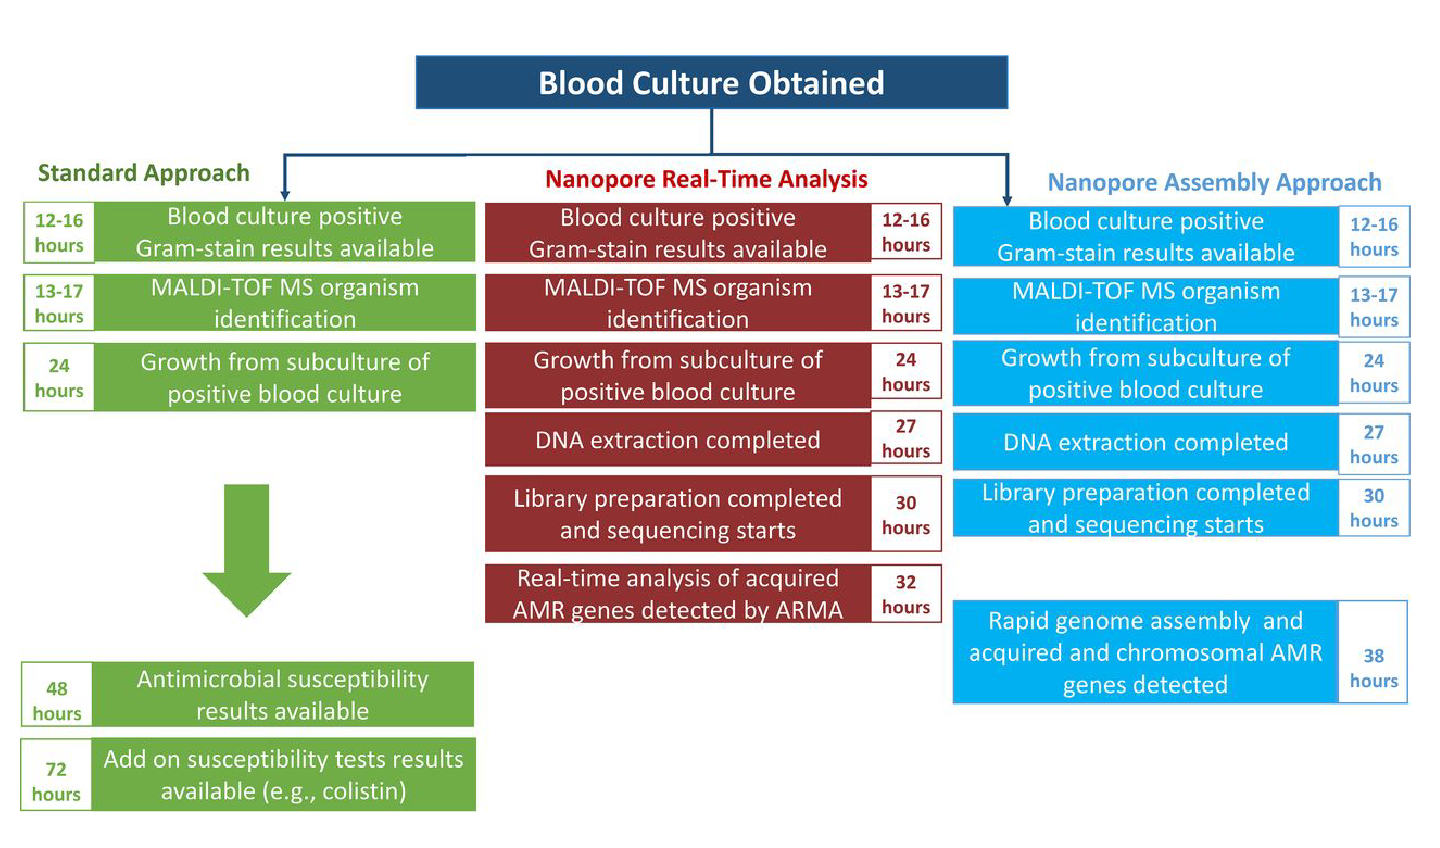
\includegraphics[width = 1\linewidth,keepaspectratio]{figure/timeline.pdf}
\caption[Estimated timelines of resistance detection]{{\bf Estimated timelines of resistance detection.} Schematic of Nanopore sequencing with a real-time analysis and assembly-based approach for identifying resistance genes compared to standard of care testing, using an example of a positive blood culture. MALDI-TOF MS, matrix-assisted laser desorption ionization<U+2013>time of flight mass spectrometry; AMR, antimicrobial resistance; AST, antimicrobial susceptibility testing. }
\label{fig:asms}
\end{figure}


\begin{table}[!hb]
\centering
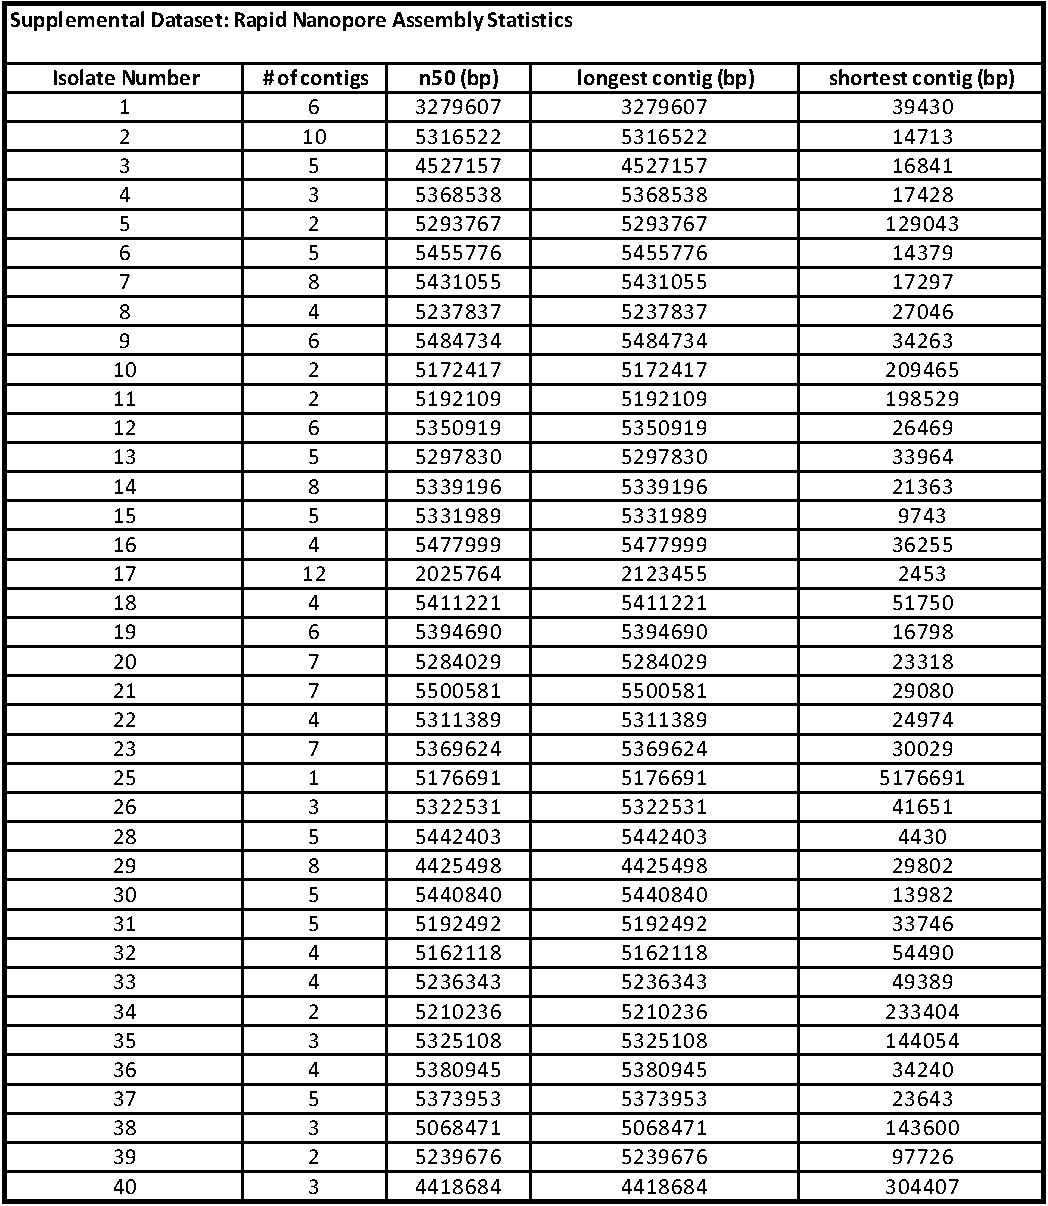
\includegraphics[width = .85\linewidth,keepaspectratio]{figure/asmrapid.pdf}
\caption[Rapid Pipeline]{{\bf Rapid Pipeline.} Assembly statistics using the rapid pipeline }
\label{tab:asmrapid}
\end{table}




\subsection{Percent agreement of WGS in predicting AST results}
\label{sec:agree}

The overall agreement of genotypic results and anticipated AST results for the 40 K. pneumoniae isolates was 77% (range, 30% to 100%), 92% (range, 80% to 100%), and 92% (range, 80% to 100%) for the Nanopore real-time approach, the Nanopore sequencing assembly approach, and the Pilon-corrected Illumina approach, respectively (Table 1). Specific details of the agreement between the predicted AST results and the broth microdilution (BMD) AST results for each of these methods are provided in Table 2 and Tables S1, S2, and S3 in the supplemental material. The Nanopore real-time approach, compared to the assembly-based approach, had an inability to identify allelic variants (i.e., blaKPC was identified but blaKPC-3 could not be specifically identified). Because all K. pneumoniae isolates are known to have chromosomally integrated non-ESBL β-lactamase genes (e.g., blaSHV-1, blaSHV-11), when blaSHV was identified, the assumption was that it was a non-ESBL blaSHV. This led to reductions in the accuracy of predictions for several β-lactams, including 5%, 2%, and 3% reductions in accurate predictions for piperacillin-tazobactam, ceftriaxone, and cefepime, respectively. Also, since the number of aminoglycoside-modifying enzymes were important to predict aminoglycoside resistance, and the alleles could not be distinguished, this led to decreases in accurate predictions for amikacin (reduced by 7%) and gentamicin (reduced by 48%). Additionally, the real-time approach was unable to identify chromosomal mutations, leading to decreases in accurate predictions for ciprofloxacin/levofloxacin (reduced by 68%) and colistin (reduced by 5%).


\subsection{Time to resistance determination}
\label{sec:time}

With a Nanopore real-time analysis approach, acquired resistance genes were identified within 8 h from subcultured isolates. Assemblies sufficient for full resistance gene and single-nucleotide polymorphism annotation using Nanopore sequences (Nanopore assembly approach) were available within 14 h from subcultured isolates. Figure 1 compares the Nanopore real-time analysis and assembly approaches with standard-of-care methods. Table 1 summarizes the agreements between antibiotic resistance determinants identified using the real-time approach, assembly-based approach, or hybrid Nanopore-Illumina assemblies and AST predictions. The following subsections describe the results summarized in Table 1 in more detail.

\subsection{Drug resistances}
\label{sec:resistance}

There were 28 ESBL genes detected in the cohort of 40 isolates. The presence of an ESBL gene (in the absence of a carbapenemase gene [n = 9]) accurately predicted resistance to ceftriaxone and aztreonam 96% of the time. There were 23 carbapenemase genes identified, including blaKPC-2 (n = 8); blaKPC-3 (n = 10); blaKPC-9 (n = 1), blaNDM-1 (n = 3), and blaOXA-48 (n = 1). The presence of a carbapenemase gene predicted meropenem and ertapenem inactivity 100% of the time and imipenem inactivity 95% of the time.

There were no isolated OmpK35 truncations identified in the absence of ESBL, AmpC, or carbapenemase-encoding genes, limiting us from better defining the contributions of inactivity of Ompk35 to β-lactam resistance. Eleven isolates had OmpK36 truncations without the coexistence of broad-spectrum β-lactamase enzymes. The presence of mutations leading to truncation of OmpK36 had poor correlation with β-lactam nonsusceptibility, ranging from 9% to 45%. Only two isolates had premature stop codons identified for both OmpK35 and OmpK36 in the absence of carbapenemase genes. Both isolates correctly predicted inactivity of ertapenem, but only one of the two isolates was resistant to meropenem and imipenem. Three isolates contained blaNDM genes. Ceftazidime-avibactam resistance was limited to these three isolates, as would be anticipated.

There were no isolates with single gyrA or parC mutations in the absence of other known fluoroquinolone resistance mechanisms, demonstrating nonsusceptibility to ciprofloxacin or levofloxacin. However, the presence of two-step gyrA mutations or gyrA mutations in conjunction with parC mutations correctly predicted fluoroquinolone resistance 100% of the time. The presence of the plasmid-mediated quinolone resistance genes qnrB or qnrS was only 50% or 33% predictive of ciprofloxacin and levofloxacin inactivity, respectively. The presence of oqxA or oqxB efflux pumps did not correlate with fluoroquinolone resistance. Finally, aac(6′)Ib-cr was associated with ciprofloxacin resistance in all three K. pneumoniae isolates in which this aminoglycoside-modifying enzyme (AME) was identified in the absence of two-step gyrA or gyrA and parC mutations.

Twenty-eight (70%) isolates produced AMEs. Aminoglycoside resistance could not be calculated a priori due to lack of clear guidance from the literature of the relationship between the number of AMEs produced and aminoglycoside resistance. In our cohort, the number of AMEs produced correlated with nonsusceptibility to gentamicin and tobramycin, with 33% of isolates being not susceptible to these agents when one enzyme was present, compared to 93% of isolates demonstrating nonsusceptibility to gentamicin or tobramycin when four or more AMEs were present (p < 0.05). Three isolates produced rRNA methyltransferases, two of these isolates also contained blaNDM-1 genes. All three isolates were resistant to gentamicin, tobramycin, and amikacin.

None of the isolates had plasmid-mediated mcr genes (mcr-1 or its variants mcr-2 to mcr-8) detected. Three isolates had colistin MICs in the non-wild-type range, all ≥8 μg/ml. For 2 of these isolates, mgrB mutations accounted for resistance using our initial prediction models. Isolate 15 had an insertion sequence IS5-like transposase that disrupted the mgrB gene, the negative regulator of the two-component regulatory system that renders polymixins ineffective (9). Isolate 22 had an elevated colistin MIC attributable to a 40-bp deletion in the mgrB gene that leads to abrogation in mgrB gene function. Finally, no mgrB mutation was identified in isolate 30. To better understand colistin resistance identified in this isolate, further investigations were performed after AST results were known. Evaluations into mutations in the two-component regulatory genes phoP and phoQ as well as pmrA and pmrB were undertaken. A deletion in phoP at position 142 resulted in a premature stop codon at amino acid 229.

The presence of trimethoprim or sulfonamide resistance genes alone correlated with trimethoprim-sulfamethoxazole resistance in 0% and 33% of isolates, respectively. Both dfr and sul genes were present in 23 isolates and correlated with trimethoprim-sulfamethoxazole resistance for 100% of isolates.

Table S4 in the supplemental material displays the average time to detection of resistance genes based on the number of reads detected in minutes. On average, one read, ten reads, 40 reads, 50 reads, and 100 reads of acquired or chromosomal genes were detected by Metrichor’s Antimicrobial Resistance Mapping Application (ARMA) in 0.6 min, 14 min, 60 min, 76 min, and 149 min, respectively.

There were 28 patients in the cohort infected with carbapenem-resistant K. pneumoniae strains. Overall, 22 (79%) received empirical antibiotic therapy that was not active against their infecting isolates. Results from Nanopore sequencing with assembly approach had the potential to place 20 (91%) of these patients on effective therapy sooner than did standard AST methods. As an example, Fig. 2 displays the timeline of a 64-year-old liver transplant recipient with a bloodstream infection caused by a K. pneumoniae isolate (isolate 29) that produced an NDM carbapenemase, CTX-M-15 ESBL, and CMY-4 AmpC β-lactamase, in addition to several mechanisms for inactivating fluoroquinolones, aminoglycosides, and trimethoprim-sulfamethoxazole. Initially, this patient was placed on standard infusion meropenem. After AST results were available and add-on testing with colistin was conducted, she was ultimately prescribed extended-infusion meropenem, colistin, and amikacin. With the use of Nanopore sequencing with assembly results, we anticipate that she potentially could have been placed on effective therapy 42 h sooner.

Overall, the median time to effective antibiotic therapy for the 28 patients infected with carbapenem-resistant K. pneumoniae was 61 h (interquartile range [IQR], 43 to 82 h). Of the antibiotics evaluated, ceftazidime-avibactam, extended-infusion meropenem, aminoglycosides, fluoroquinolones, polymixins, and tigecycline are generally considered reasonable treatment options for infections caused by carbapenem-resistant K. pneumoniae isolates, if active in vitro. As results from the real-time analysis approach were generally available within 8 h from subcultured isolates, Nanopore real-time analysis could have led to an average time to effective therapy of 41 h (IQR, 33 to 44). Using the Nanopore assembly approach, time to effective therapy could have been reduced to 35 h (IQR, 32 to 42). The time to effective therapy was reduced with the assembly approach compared to that with the real-time approach because the former provided more comprehensive data to infer AST activity (e.g., aminoglycoside resistance, colistin resistance, etc.) than the real-time approach, for which there were delays in antibiotic optimization while awaiting additional AST results. Both the real-time and assembly approaches were significantly faster than the standard approach (p < 0.05).

\section{Discussion}
\label{sec:discuss}

Our results demonstrate that Nanopore sequencing can be employed to both accurately and rapidly predict phenotypic AST profiles. Our study builds off previously published proof-of-concept or early insight studies applying Nanopore sequencing for the detection of antimicrobial resistance genes (8, 10–16). We found an overall agreement of 92% between genotypic results and comprehensive AST results using a Nanopore assembly-based approach. We further demonstrated that assembly-based approaches enhance the ability to identify chromosomal mutations and allelic variants compared to that of the Nanopore real-time approach. A future method centered on real-time alignment and consensus of raw reads to a database of antimicrobial resistance (AMR) genes will enhance the capabilities of the real-time approach. Nevertheless, even with its current limitations, the Nanopore real-time analysis approach correctly predicted the presumed activity of a number of antibiotics commonly prescribed for Gram-negative infections, such as β-lactams, trimethoprim-sulfamethoxazole, tetracyclines, with reasonable accuracy, with full annotation of acquired AMR genes within 8 h from the time of cultured isolates. Within 14 h of cultured isolates, a Nanopolished assembly-based approach would allow for predictions of the activity of additional agents, such as fluoroquinolones, aminoglycosides, and polymixins (beyond mcr-1 and its variants), due to the ability to detect chromosomal mutations or allelic variants leading to resistance. We believe that with rapid extraction and library preparation techniques, the turn-around times could further be reduced to ≤3 h for a real-time approach and ≤9 h for a Nanopore assembly-based approach. Moreover, using a hypothetical trial design, we found that a real-time approach and assembly approach could shorten the average time to effective antibiotic therapy for carbapenem-resistant K. pneumoniae infections by 20 h and 26 h, respectively, compared to standard approaches.

Although there have been other investigations of the use of WGS to predict AST results for Gram-negative organisms based on resistance determinants (2, 5–8, 10–13, 16), ours is the first to use a Nanopore assembly approach for evaluating a broad range of acquired resistance genes and chromosomal mutations in predicting susceptibility results for a comprehensive panel of antibiotics. Previous studies applying Nanopore sequencing for resistance gene detection have applied this methodology to small numbers of isolates and limited evaluations to acquired resistance genes. Furthermore, the potential impact of WGS in reducing time to appropriate antibiotic therapy for highly drug-resistant organisms has not been previously reported. As the science of WGS continues to evolve, the costs of sequencing are becoming more affordable, and the time requirements for DNA extraction, library preparation, assembly, and detection are anticipated to be further reduced. We believe that this methodology can accurately expedite antibiotic decision making for critically ill patients infected with MDRGN organisms. WGS also provides the ability to identify emerging mechanisms of resistance, such as mcr variants or novel mechanisms of resistance against newly approved agents (17, 18).

As we continue to gain further insights into the complexities of resistance mechanisms present in Gram-negative organisms, it is becoming increasingly clear that sole reliance on the detection of β-lactamase genes to identify antibiotic resistance is insufficient. Such is the case with commercially available PCR-based methodologies (e.g., Cepheid Xpert Carba-R assay, BioFire FilmArray blood culture identification panel, Verigene Gram-negative blood culture test, etc.) that fail to identify the wide array of additional resistance determinants (e.g., porin deletions, multidrug efflux pumps, functioning of the two-component regulatory system, DNA gyrase mutations, off-panel targets, etc.). Using carbapenem-resistant K. pneumoniae as a case study, over half of isolates render carbapenem antibiotics ineffective due to non-carbapenemase-mediated mechanisms (4). Similarly, carbapenem resistance among Pseudomonas aeruginosa strains in the United States is predominantly mediated by noncarbapenemase mechanisms, including the loss of OprD porin expression and/or upregulation of MexAB-OprM efflux pumps (19). WGS offers a more comprehensive approach to identifying clinically relevant antibiotic resistance compared with standard PCR technologies.

Nanopore technology offers real-time DNA sequencing of long reads, which facilitate the process of high-quality genome assembly (20). Additionally, they are better able to capture large regions of structural variation (e.g., insertions, deletions, duplications, translocations, inversions, etc.) and resolve repetitive regions accurately, compared to technologies which generate short-read data. However, there are some drawbacks to Nanopore sequencing (20). Chromosomal mutations as small as single-base polymorphisms in DNA can result in drastic changes to proteins due to frame shifts or early truncations. Indels and resulting false positives in chromosomal mutations can be difficult to distinguish with Nanopore sequencing alone (21). The assembly process generally removes random error, given sufficient sequencing coverage. However, systematic errors in the form of homopolymer indels and methylation errors still result in disagreement compared with Illumina-corrected assemblies. Nanopolish corrects most homopolymer indels, improving accuracy, but in its current form, it is not all-inclusive (22). Methylation motifs alter the electrical signal from Nanopore sequencing, resulting in errors in base calling. We anticipate further improvements to the quality of Nanopore sequencing and available bioinformatics, enabling this technology to rapidly and accurately resolve variants of acquired resistance genes and characterize chromosomal mutations in the absence of assembly.

We assessed the minimum sequencing time to be able to accurately predict AST using Nanopore sequencing. We determined that a minimum of 10 reads per gene were required and that a sequencing run of 1 h is sufficient to predict the AST profile, using either a real-time ARMA or an assembly approach. In fact, we were able to detect 10 reads of all AMR genes within 14 min of starting the sequencing run and 40 reads of each gene within 1 h. This is an important quality control measure as we begin to consider these methods for clinical application.

There are several remaining limitations to this work. First, there were some antimicrobial susceptibility profiles for which we were unable to identify the associated resistance mechanisms, suggesting that our approach to resistance detection was not comprehensive. As an example, we were only able to accurately predict piperacillin-tazobactam activity 85% of the time. This is similar to what others have shown (2), and it is likely due to efflux pumps, where expression analysis is required. Second, there were some agents tested for which no resistance was observed (e.g., tigecycline), precluding us from including these agents in our analysis. Third, we only evaluated K. pneumoniae isolates from a single region of the United States. Validation needs to occur in larger data sets with a more diverse array of genera and species and resistance mechanisms, including some not observed in our isolates, such as the mcr genes. Additionally, as antibiotic susceptibility criteria include several considerations, such as wild-type MIC distributions, pharmacokinetic-pharmacodynamic modeling, clinical outcomes data, etc., it can be challenging to determine the most accurate MIC that signifies nonsusceptibility. The European Committee on Antimicrobial Susceptibility Testing suggests that epidemiologic cutoff values (i.e., wild-type versus non-wild-type distributions) are the preferred values for correlation with resistance genes (23). We elected to use antibiotic breakpoints, as these remain the most relevant metric for quantifying antibiotic resistance for clinicians, but we realize that this might not be the most accurate proxy.

In conclusion, we were able to leverage the long reads, rapid turnaround time, and real-time analytic capabilities of Nanopore sequencing to accurately identify resistance loci. With the continued rise in highly drug-resistant infections, the need for rapid and accurate methods to detect antibiotic resistance is becoming increasingly important. Continued enhancements to WGS may permit real-time AMR gene detection from clinical isolates in the near future.

\section{Materials and Methods}
\label{sec:methods}

\subsection{Study cohort}
\label{sec:cohort}

Forty clinical Klebsiella pneumoniae complex isolates collected between 2016 and 2017 and processed at the Johns Hopkins Hospital Medical Microbiology Laboratory were included in the present study. Isolates for inclusion were deliberately selected based on their diversity of AST results and mechanisms of resistance and included 30 carbapenem-resistant (21 carbapenemase producers and 10 non-carbapenemase producers) and 9 carbapenem-susceptible K. pneumoniae isolates. As this was a proof-of-concept study comparing different WGS approaches, we decided to focus on a single genus and species (i.e., K. pneumoniae) to increase the number of isolates with any single resistance mechanism identified, as some resistance mechanisms are genus and species specific, especially among chromosomal mutations leading to resistance. Isolates were subcultured from frozen stock to tryptic soy agar (TSA) with 5% blood agar. A second subculture was performed prior to DNA extraction. K. pneumoniae isolates from deep tissue (n = 3), intraabdominal fluid (n = 1), blood (n = 10), respiratory (n = 10), and urine (n = 16) were included.

\subsection{Species and antimicrobial susceptibility testing}
\label{sec:ast}

Bacterial genus and species were identified using matrix-assisted laser desorption ionization–time of flight mass spectrometry (Bruker Daltonics Inc., Billerica, MA). AST results were determined using the BD Phoenix Automated System NMIC-303 panels (BD Diagnostics, Sparks, Maryland). MICs were confirmed by broth microdilution (BMD) with Sensititre GNX2F Gram-negative panels (Thermo Fisher Scientific, Indianapolis, IN) and the ceftazidime-avibactam Etest (bioMérieux, France) (24). BMD was repeated on isolates with 2-fold or greater MIC discrepancies between the Phoenix automated panel and initial BMD results. Interpretive criteria established by the Clinical and Laboratory Standards Institute (CLSI) were used to define antibiotic susceptibility (25). AST results in both the “intermediate” and “resistant” ranges were categorized as resistant.

\subsection{Whole-genome sequencing and antimicrobial resistance gene detection}
\label{sec:wgs}

As Nanopore sequencing has a substantial raw sequencing error rate, three separate sequencing and analysis pipelines were performed, as follows: (i) a real-time Nanopore (Oxford, England) analysis approach that identified acquired and chromosomal resistance genes by applying Metrichor’s Antimicrobial Resistance Mapping Application (ARMA) (https://nanoporetech.com/resource-centre/real-time-detection-antibiotic-resistance-genes-using-oxford-nanopore-technologies); (ii) an assembly-based Nanopore approach that uses Canu and Nanopolish (22, 26) to compute high-identity sequences with identification of resistance genes, using Abricate ResFinder results as well as chromosomal mutations (e.g., ompK35 and ompK36 mutations, gyrA and parC mutations, etc.) from genomic assemblies, using minimap2 and a novel tool evaluating the impact on amino acid translation based on resulting codon changes (27, 28); and (iii) a Pilon-corrected hybrid approach using both Illumina (Illumina, San Diego, California) and Nanopore sequencing (29). The short-read correction of Nanopore assemblies served as the reference standard to determine the accuracy of Nanopore sequencing results. A detailed description of the sequencing and analysis methods is included in supplemental material (Supplemental Data Set S1).

\subsection{Predicted correlations between WGS and AST results}
\label{sec:wgsast}

Predictions of resistance were performed without reference to phenotypic data, unless otherwise noted in Results. The correlations of resistance genes and sequence variants with anticipated AST results for the evaluated antibiotics were determined based on reference gene databases and the published literature (30–47; see also K. Bush, T. Palzkill, and G. Jacoby, http://www.lahey.org/studies/). Antimicrobial resistance genes and mutation results were reviewed manually to predict AST results. Details on the predictive models applied to chromosomal mutations and acquired resistance genes to predict phenotypic AST can be found in the supplemental material.

\subsection{Clinical data}
\label{sec:clinical}

An infectious diseases physician (P.D.T.) confirmed all isolates to be representative of clinical infections by manual chart review. Detailed clinical and treatment data were collected to identify if the time to effective antibiotic therapy would have decreased had Nanopore sequencing data with a real-time analysis approach or an assembly-based approach been used in predicting AST results compared to that with standard AST identification methods. Dates and times antibiotic regimen changes occurred and the timing of the availability of clinical culture results were recorded. Furthermore, time points for the steps involved in Nanopore sequencing and identification of resistance determinants were also recorded. The Johns Hopkins University School of Medicine Institutional Review Board approved this study, with a waiver of informed consent.

\subsection{Data Availability}
\label{sec:avail}

Sequencing data for this study were deposited in the Sequence Read Archive (BioProject number PRJNA496461).
